\documentclass{paper}[11pt]
\usepackage{geometry}
\usepackage{amsmath}
\usepackage{graphicx}
\usepackage{braket}
\usepackage{enumitem}
\usepackage{amssymb}
\usepackage{hyperref}
\usepackage{titling}
\usepackage{parskip}
\usepackage{subcaption}



\title{Calibration and Troubleshooting}

\author{Lev Gruber}

\date{7/11/2024}

\begin{document}
\maketitle 

\tableofcontents
\newpage
\section{Introduction}
You're starting the do work with Professor Lynn's Quantum Optics Group at Harvey Mudd College; congrats! It's a super cool lab doing fascinating research, and I am sure you'll have an amazing time. The only road blocks ahead are random bugs, apparatus errors, and worst of all, when you have to recalibrate everything from scratch. This guide, much of it adapted or copied from Alec Roberson's work \textit{How to Calibrate Everything} in the GitHub's Summer 2023 repo, provides fixes for these issues. Please reference Alec's write up for more information on \textit{why} the calibration procedure works, as this guide will focus more so on what actions to take. Alec's guide also contains literature on Jones' matrices, laser drift, and other useful topics that I won't copy verbatim for this document. Therefore, I fully recommend you read through 
\textit{How to Calibrate Everything} if you're struggling through the calibration from scratch.

\section{Calibration from Scratch}
Some important notes before you begin calibration include:
\begin{itemize}
    \item Remember to always wear goggles when the laser is unblocked, to never turn on the lights unless the detectors are off, and to never look down the path of the laser. It is ok to remove your goggles when sitting behind the computer due to the screen and elevation. 
    \item DO NOT look down the path of the laser, and do not have your eyes level with the optical axis. This holds true whether or not you have goggles on.
    \item DO NOT turn off the computer, or else you may have to reassign every motor to its corresponding port. 
    \item The black motors with the tick marks are Thorlabs motors and the red motors with no tick marks are Elliptec motors.
    \item The Thorlabs motors are controlled by the software 'APT User', and the Elliptec motors 'Ello'.
    \item If power is lost, Thorlabs motors will assume their new 'zero' is wherever they were when they lost power. Calibration in the config.json is based off of the Thorlabs motors at their visual zero, so visual zero is a good guess at calibration (to be close to previous values for a new calibration). Oppositely, we have no clue what the Elliptec motor thinks zero is post-power loss--our best guess is np.random.rand().
    \item All calibration files calibrate by sweeping a wave plate, or moving it while seeing how counts changes in a specific basis. Ensure that the sweep parameters are set to be at minimum 8 degrees above and below the previously calibrated value in the config for a given wave plate. 
\end{itemize}

\subsection{The Quartz Plate (QP)}
First, we need to calibrate the quartz plate. Open 'Ello' on the computer, select COM12 in the upper left, and hit connect. See the tab denoted with address A. You can jog the motor to ensure you've selected the QP. 

Note: \textbf{Wear goggles and do not look down the path of the laser.}

Turn off the lights, unblock the laser (wear goggles!), and use a business card or small piece of paper to identify the light reflecting off of the QP back towards the mirrors and laser. Each element in the apparatus' state creation section retroreflects, so use a second business card to ensure you're looking at the correct reflection; this can be done by holding one business card with the potential retroreflection showing, then using a second business card to block the laser's path before or after the QP. If the retroreflection disappears when the business card is placed after the QP, you have the wrong retroreflection. If it disappears when placed before (and not after) the QP, then you have identified the correct retroreflection. Begin with the QP visually perpendicular with the incoming light, and jog it slightly CW or CCW until a portion of the incoming beam retroreflects directly below the incoming beam on the laser's front. Note this will be directly below the outgoing laser due to table slant.

Once retroreflecting correctly, update the home offset within Ello by adding the current offset to the current position; if the result is negative, add 360. 

\subsection{Alice's Wave Plates (and the UV Half Wave Plate)}
We begin measurement-side calibration with Alice's side. Open VS Code and go to the calibration folder and within that, AQWP.py (Alice quarter wave plate). For this we also need to remove Bob's PBS and Alice's half wave plate; both are on magnetic stands so can be carefully pulled off at the base and placed out of the laser's path. Be incredibly gentle so as to not loosen the PBS from its holder. After removing, run the file. The minima of the resulting curve is where the calibrated AQWP zero should be. Add this to the current value for AQWP in the config.json. It should look something like figure \ref{fig:AQWP}.

Next is the UV half wave plate (UVHWP), so navigate to that folder and run UVHWP.py--the parabola minimum is where you should update the config to (plus the original config value), as in figure \ref{fig:UVHWP}. There is no way to tell when the UV HWP is close to a previous calibration, so you will need to sweep a large range of ~45 degrees. 

Moving to Alice's half wave plate (AHWP), put it back into the set up, then run AHWP.py. Once again, the minimum value should be added to the current config.json value and config.json saved. This should look like \ref{fig:AHWP}

Finally, run check.py within the checka folder. This sweeps all plates around their calibrated zeros (does a minisweep) to ensure all are calibrated correctly. We aim for a $< 0.1$ degree error on each plate, meaning the measured zero is within 0.1 degree of the calibrated zero in the config. You may have to run this a few times, updating the wave plates each time, to converge with low error. 
\begin{figure}[t]
    \centering
    \begin{subfigure}{0.32\linewidth}
        \centering
        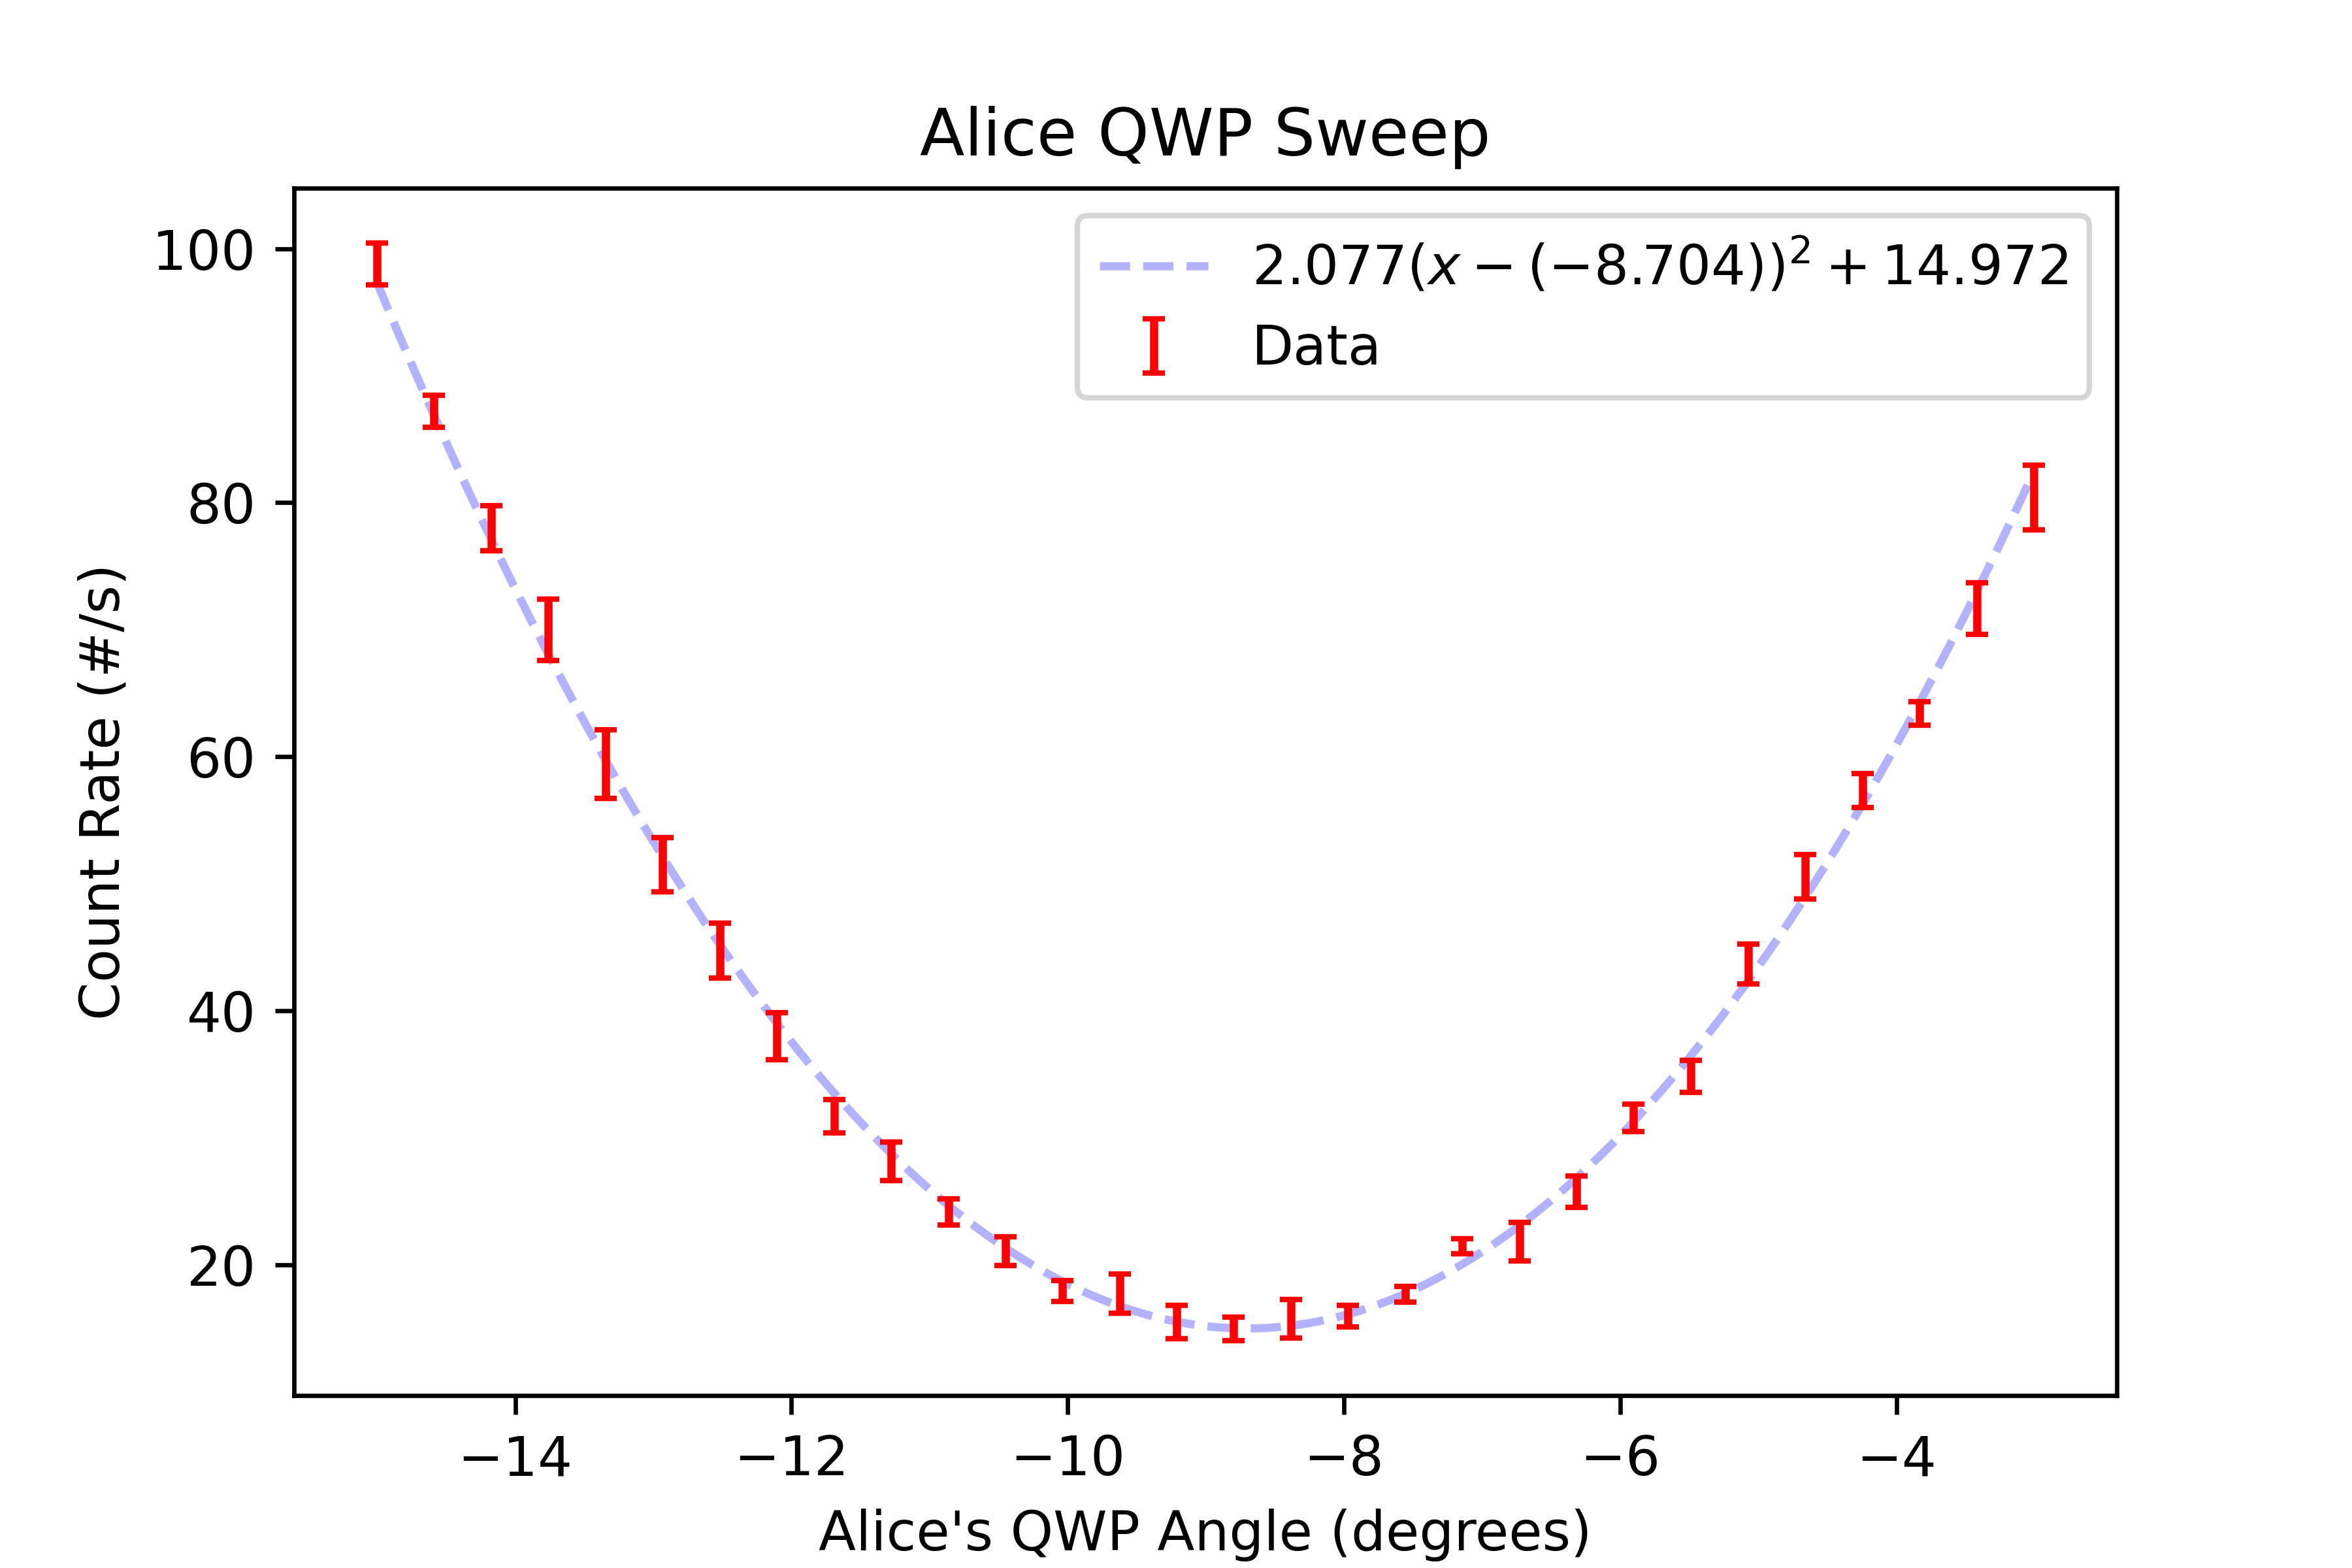
\includegraphics[width=1\linewidth]{figs/AQWP_sweep2.png}
        \caption{}
        \label{fig:AQWP}
    \end{subfigure}
    \begin{subfigure}{0.32\linewidth}
        \centering
        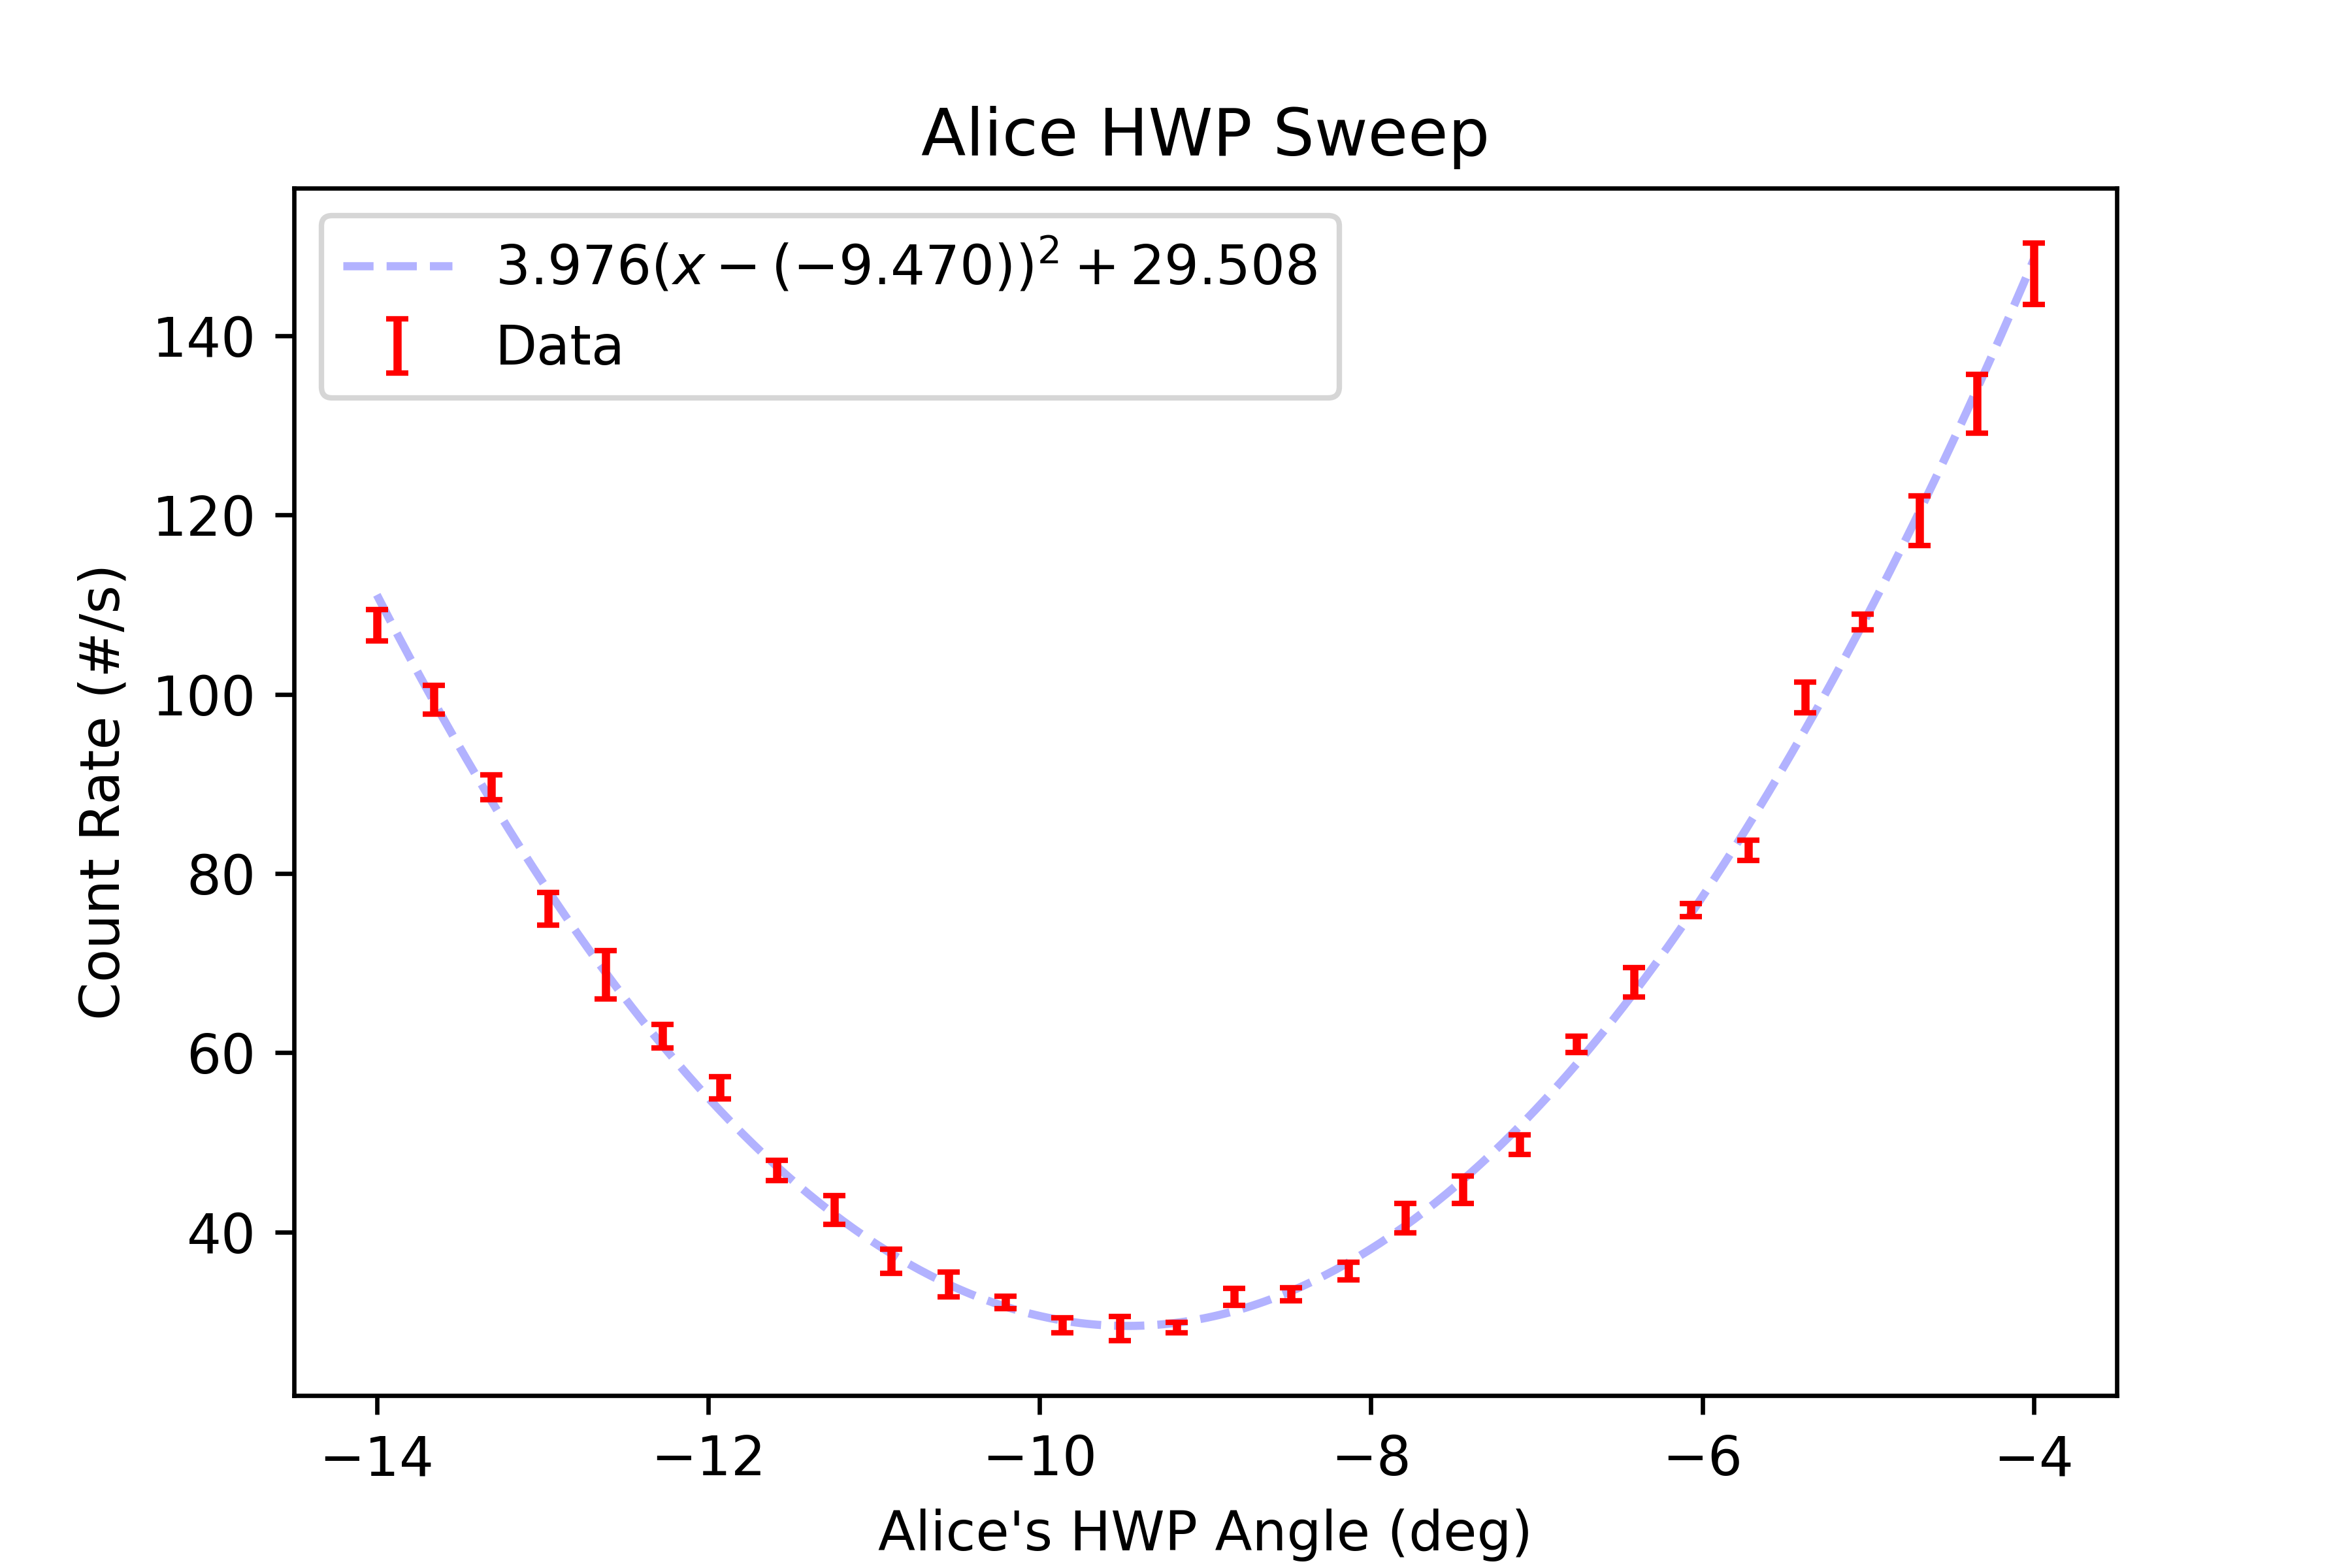
\includegraphics[width=1\linewidth]{figs/AHWP_sweep1.png}
        \caption{}
        \label{fig:AHWP}
    \end{subfigure}
    \begin{subfigure}{0.32\linewidth}
        \centering
        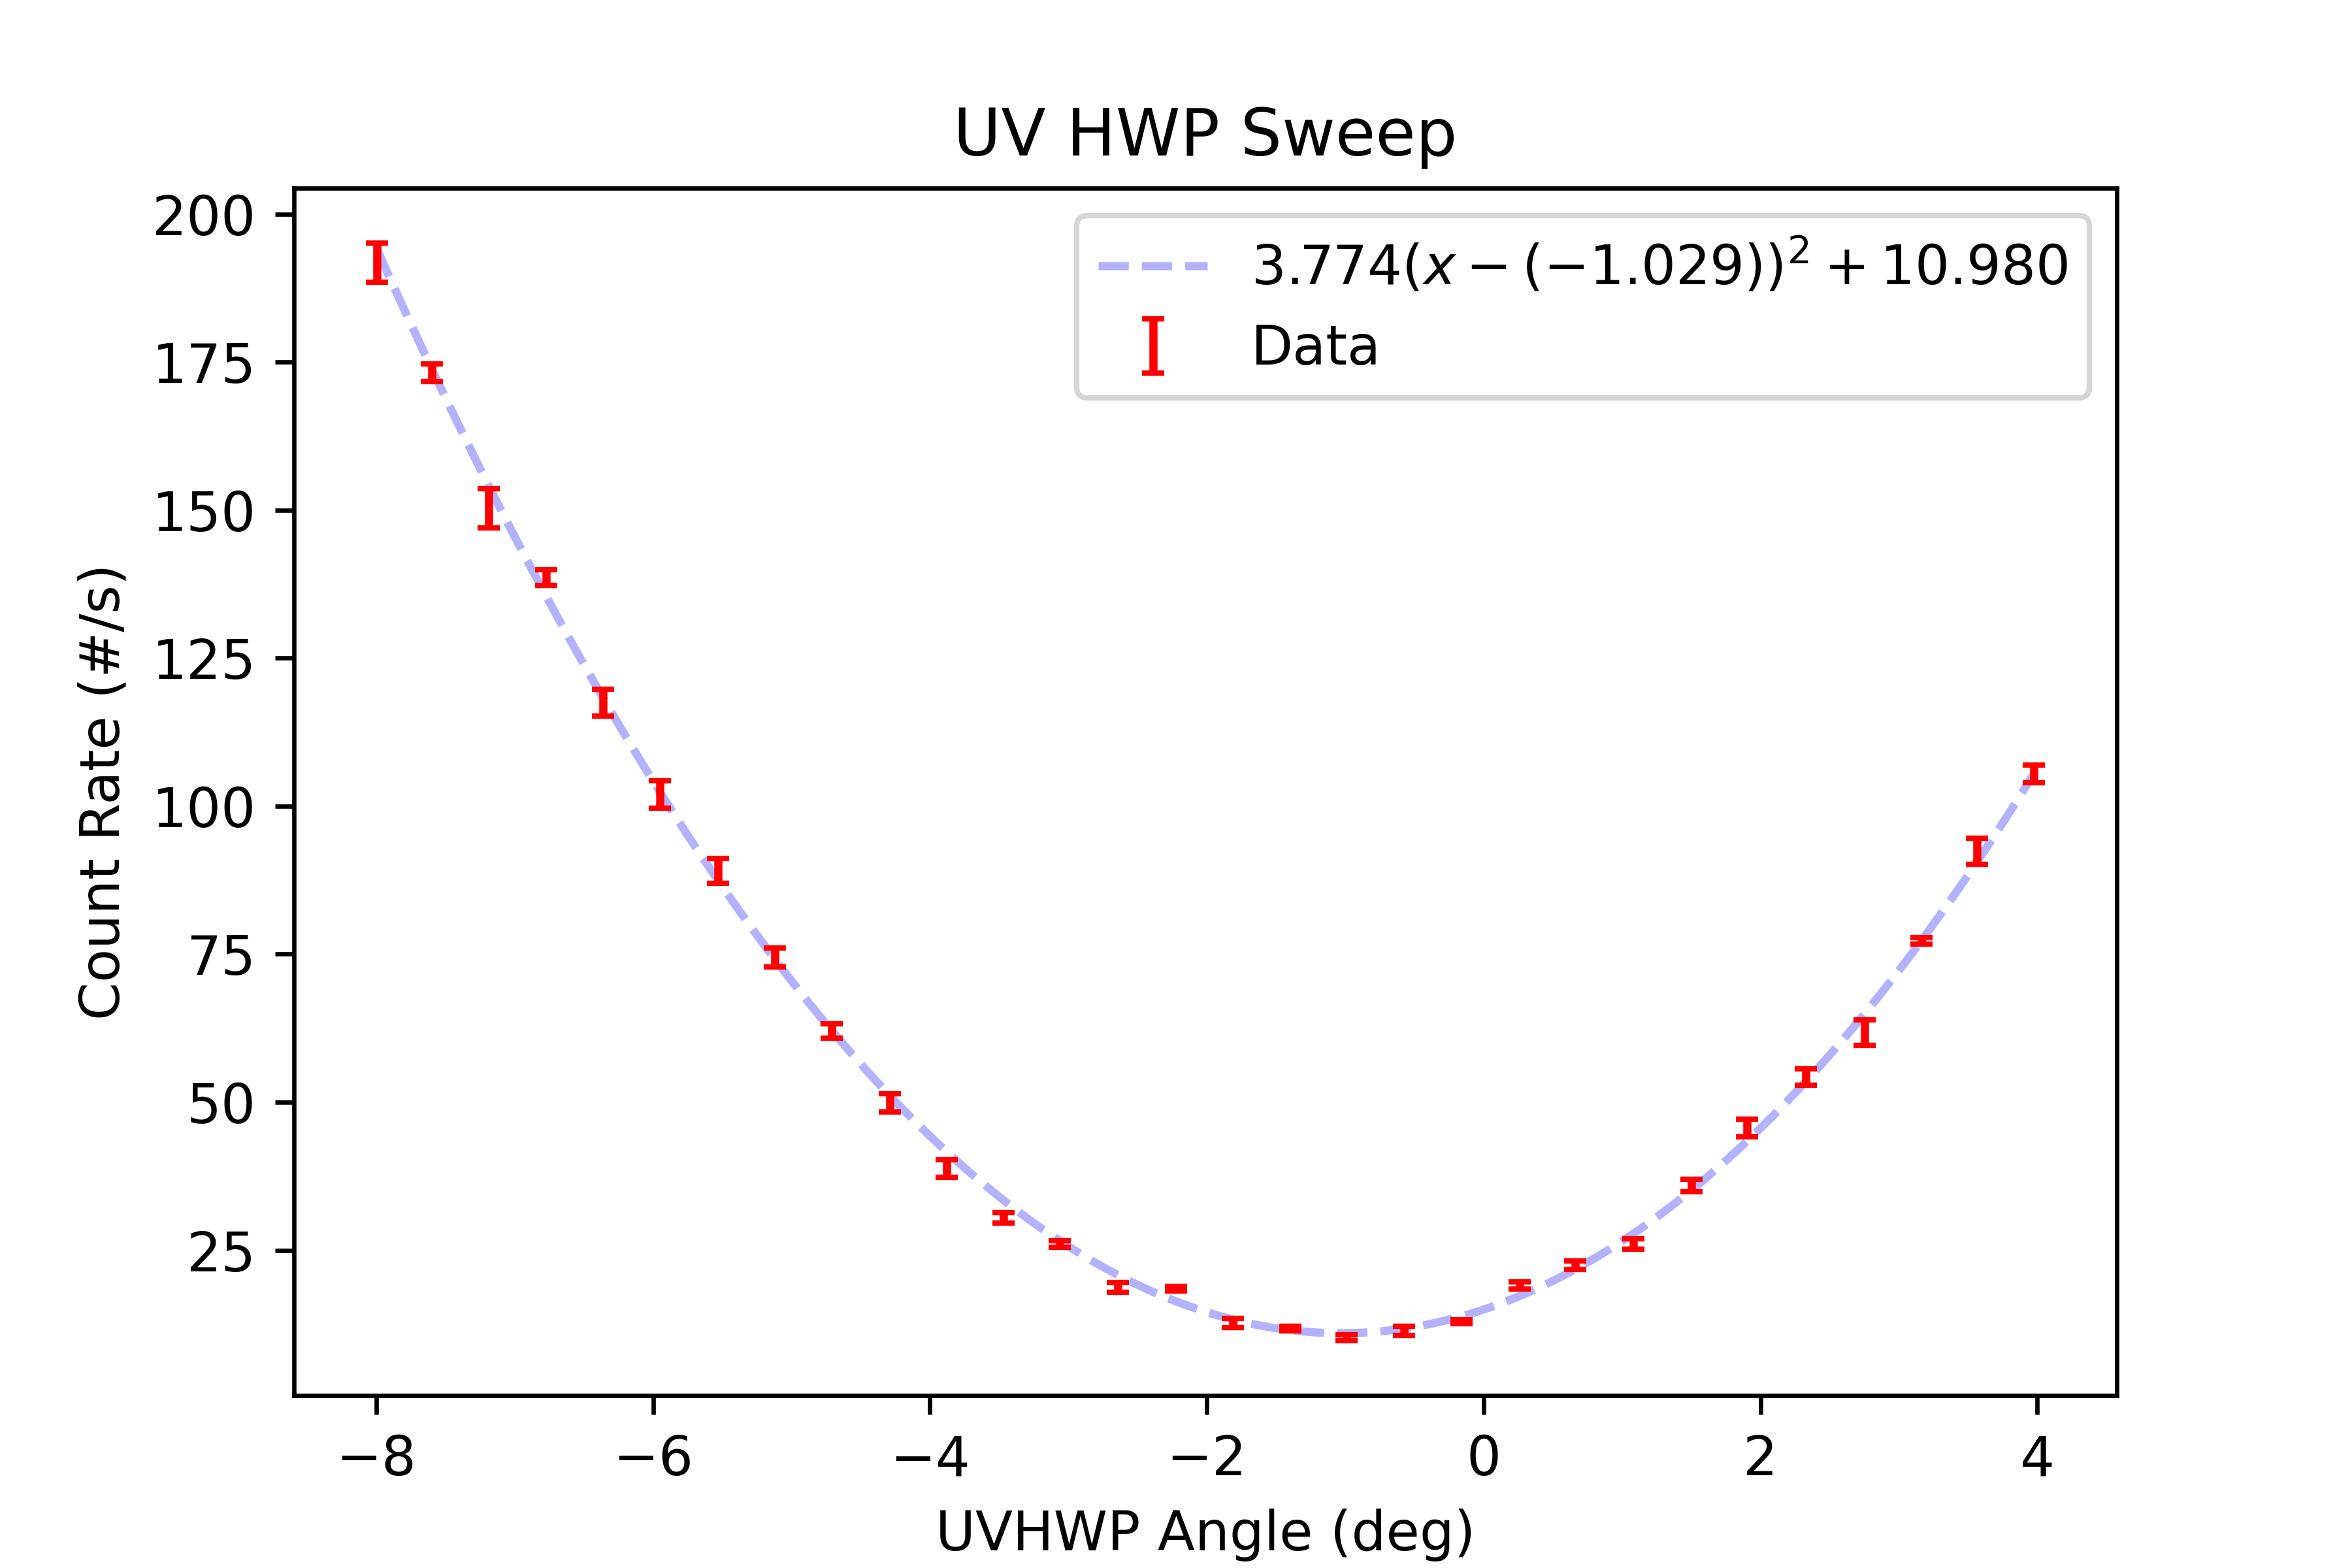
\includegraphics[width=1\linewidth]{figs/UVHWP_sweep1.png}
        \caption{}
        \label{fig:UVHWP}
    \end{subfigure}
    \caption{Left to right: AQWP calibration curve, AHWP calibration curve, UV HWP calibration curve}
\end{figure}

\subsection{Bob's Wave Plates}
The first step is to reinsert Bob's PBS--be careful not to jog the crystal out of place. Then remove Bob's creation half wave plate (BCHWP), Bob's half wave plate (BHWP), and Bob's creation quarter wave plate (BCQWP). BCHWP is screwed down, with tape markings where it should be re-inserted later, as is BCQWP. It can be unscrewed and gently moved out of the photon's path. BHWP is on a magnetic mount, and can be gently removed from the mount at the base and placed out of the photon's path. 

Begin with Bob's Quarter Wave Plate (BQWP)--run the sweep using BQWP.py and update the config accordingly. An example is shown in figure \ref{fig:BQWP}. 

Next is BCHWP, which should be screwed into the table following the tape guidelines. Sweep and update the config, the plot looking as in figure \ref{fig:BCHWP}.

Then, reinsert BHWP onto the magnetic mount gently, and run BHWP.py. You should get a plot like \ref{fig:BHWP}; update the config accordingly. 

Run check.py within checkb, which has the same functionality as Checkpoint A but for Bob's side. This functions as a final check that our measurement side is calibrated correctly. Again, it may be an iterative process to converge on a calibration with $0.1$ deg uncertainty.

Finally, carefully reinsert BCQWP and run its corresponding calibration file BCQWP\_calibration.py within BCQWP/BCQWP\_Stu. You should receive back a parabola, the minima of which should be added to the current calibration in config.json. This looks like figure \ref{fig:BCQWP}.

\begin{figure}
    \centering
    \begin{subfigure}{0.35\linewidth}
        \centering
        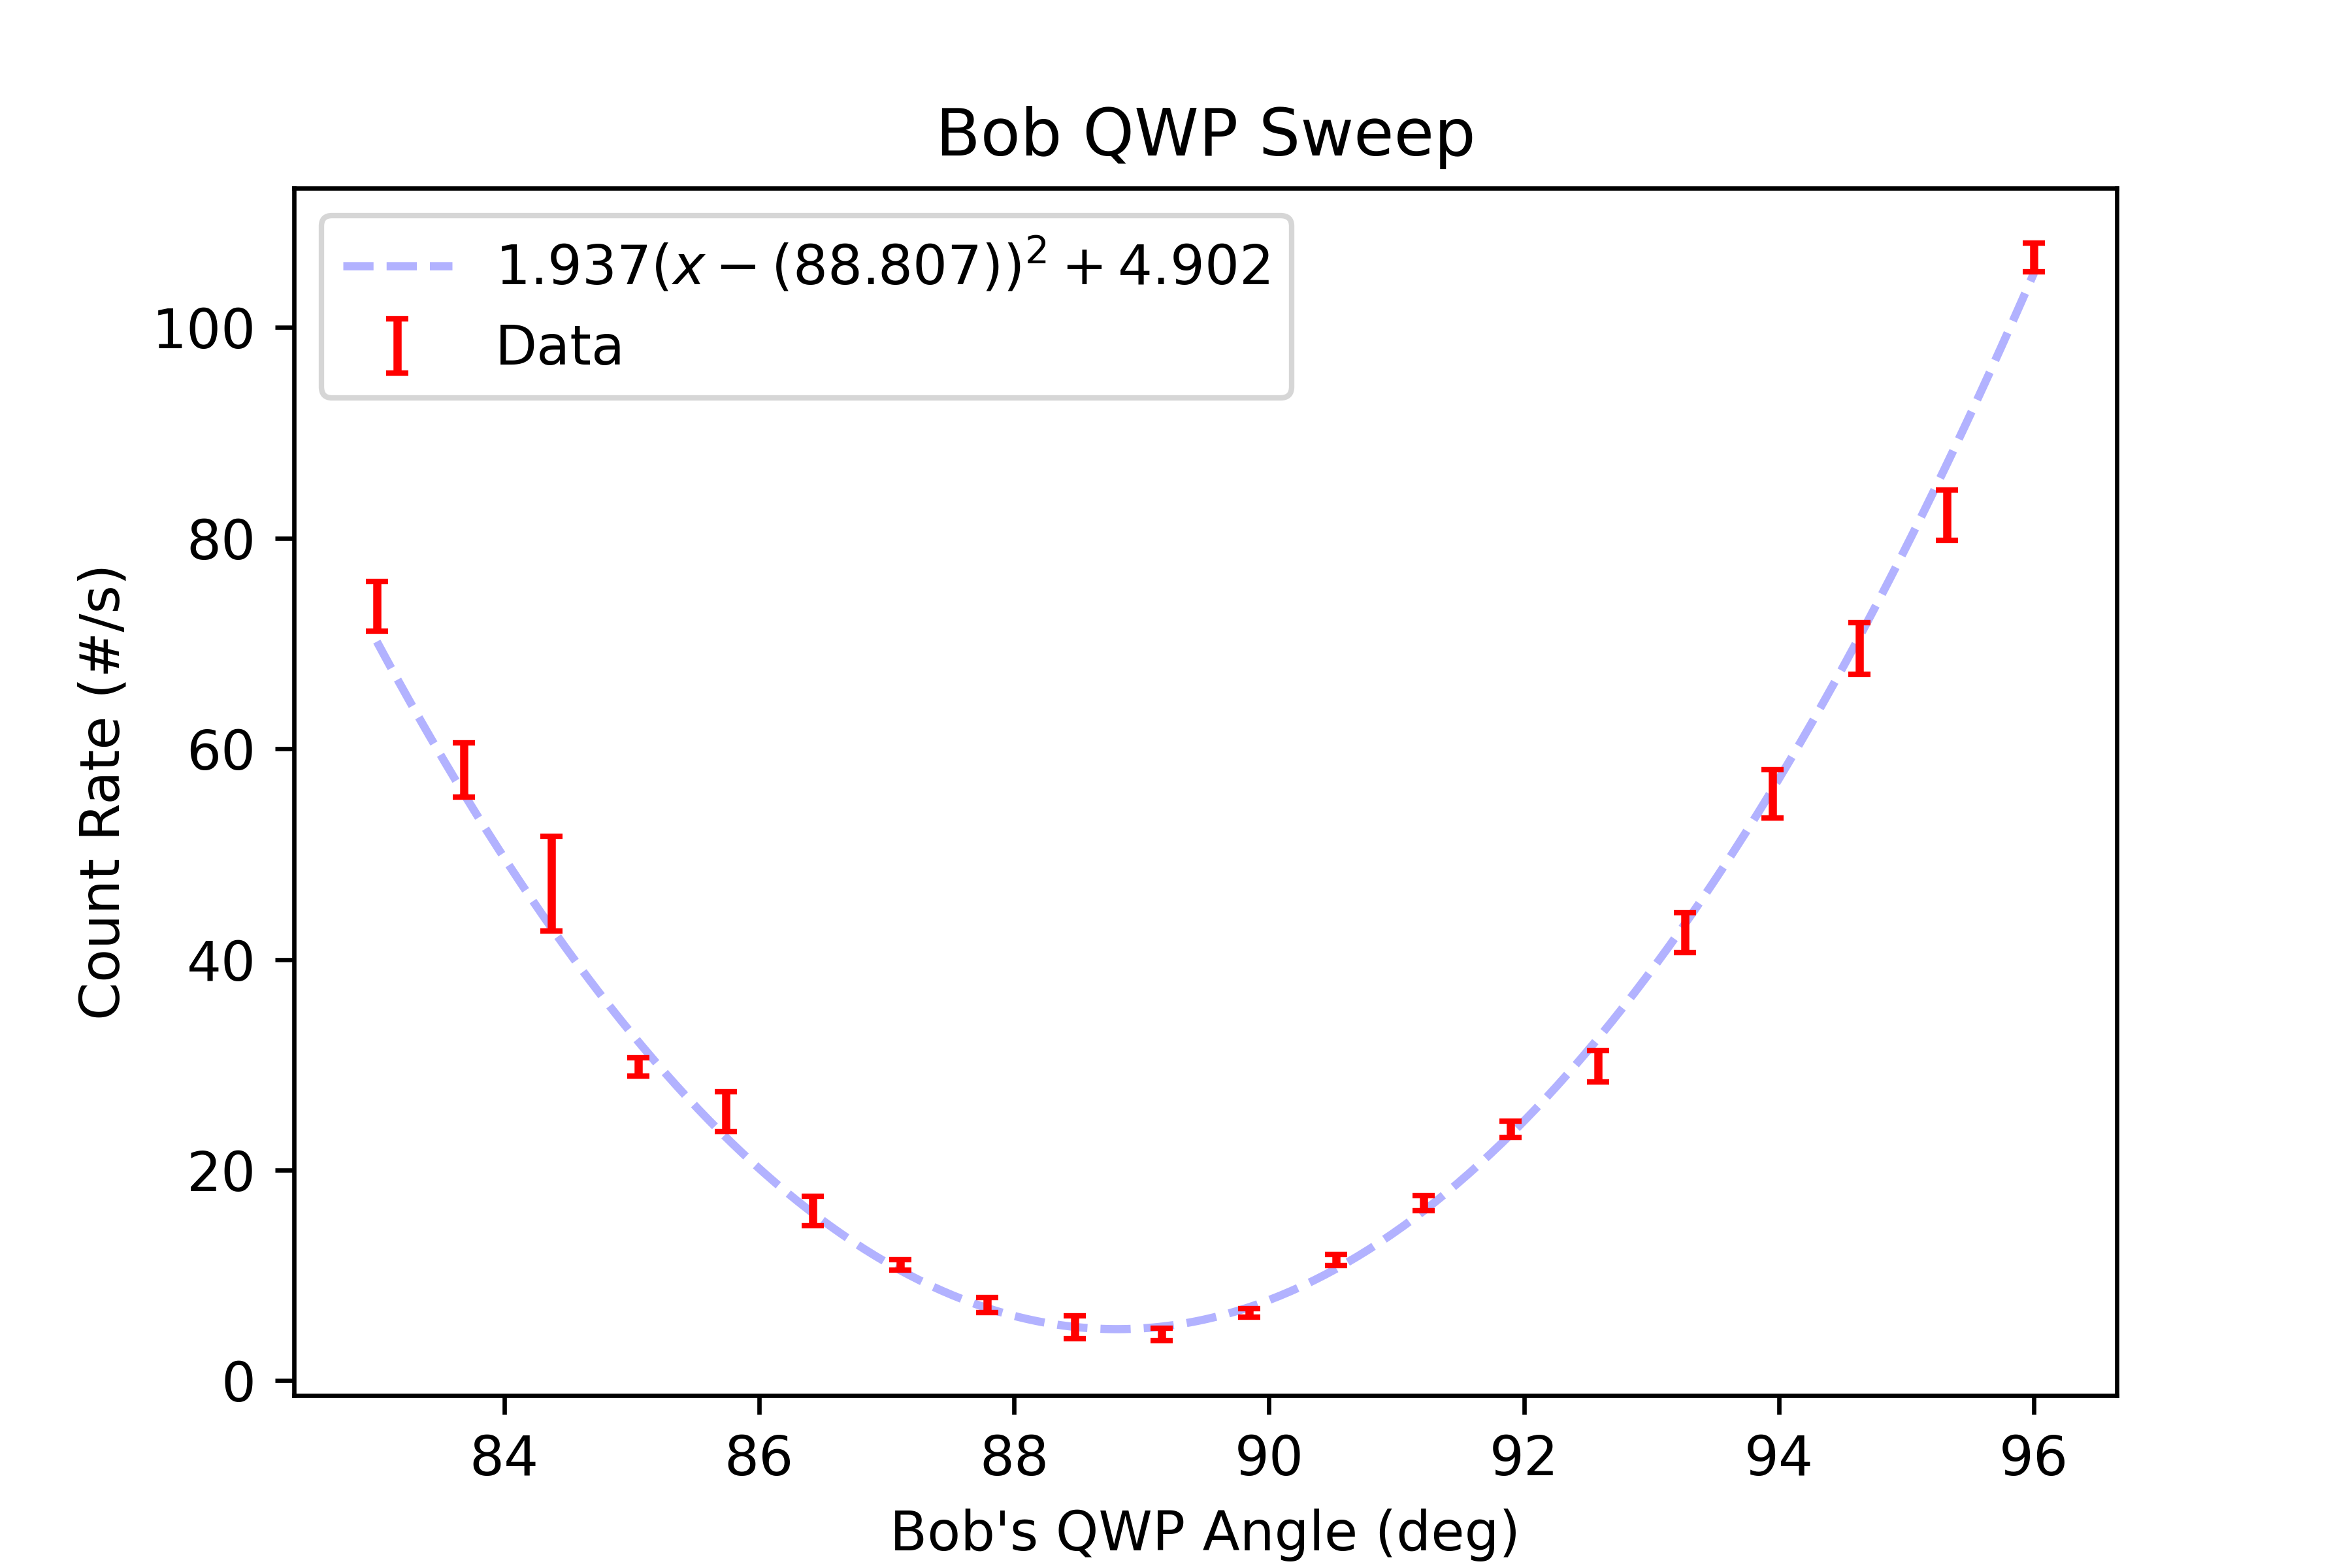
\includegraphics[width=1\linewidth]{figs/BQWP_sweep0.png}
        \caption{}
        \label{fig:BQWP}
    \end{subfigure}
    \begin{subfigure}{0.35\linewidth}
        \centering
        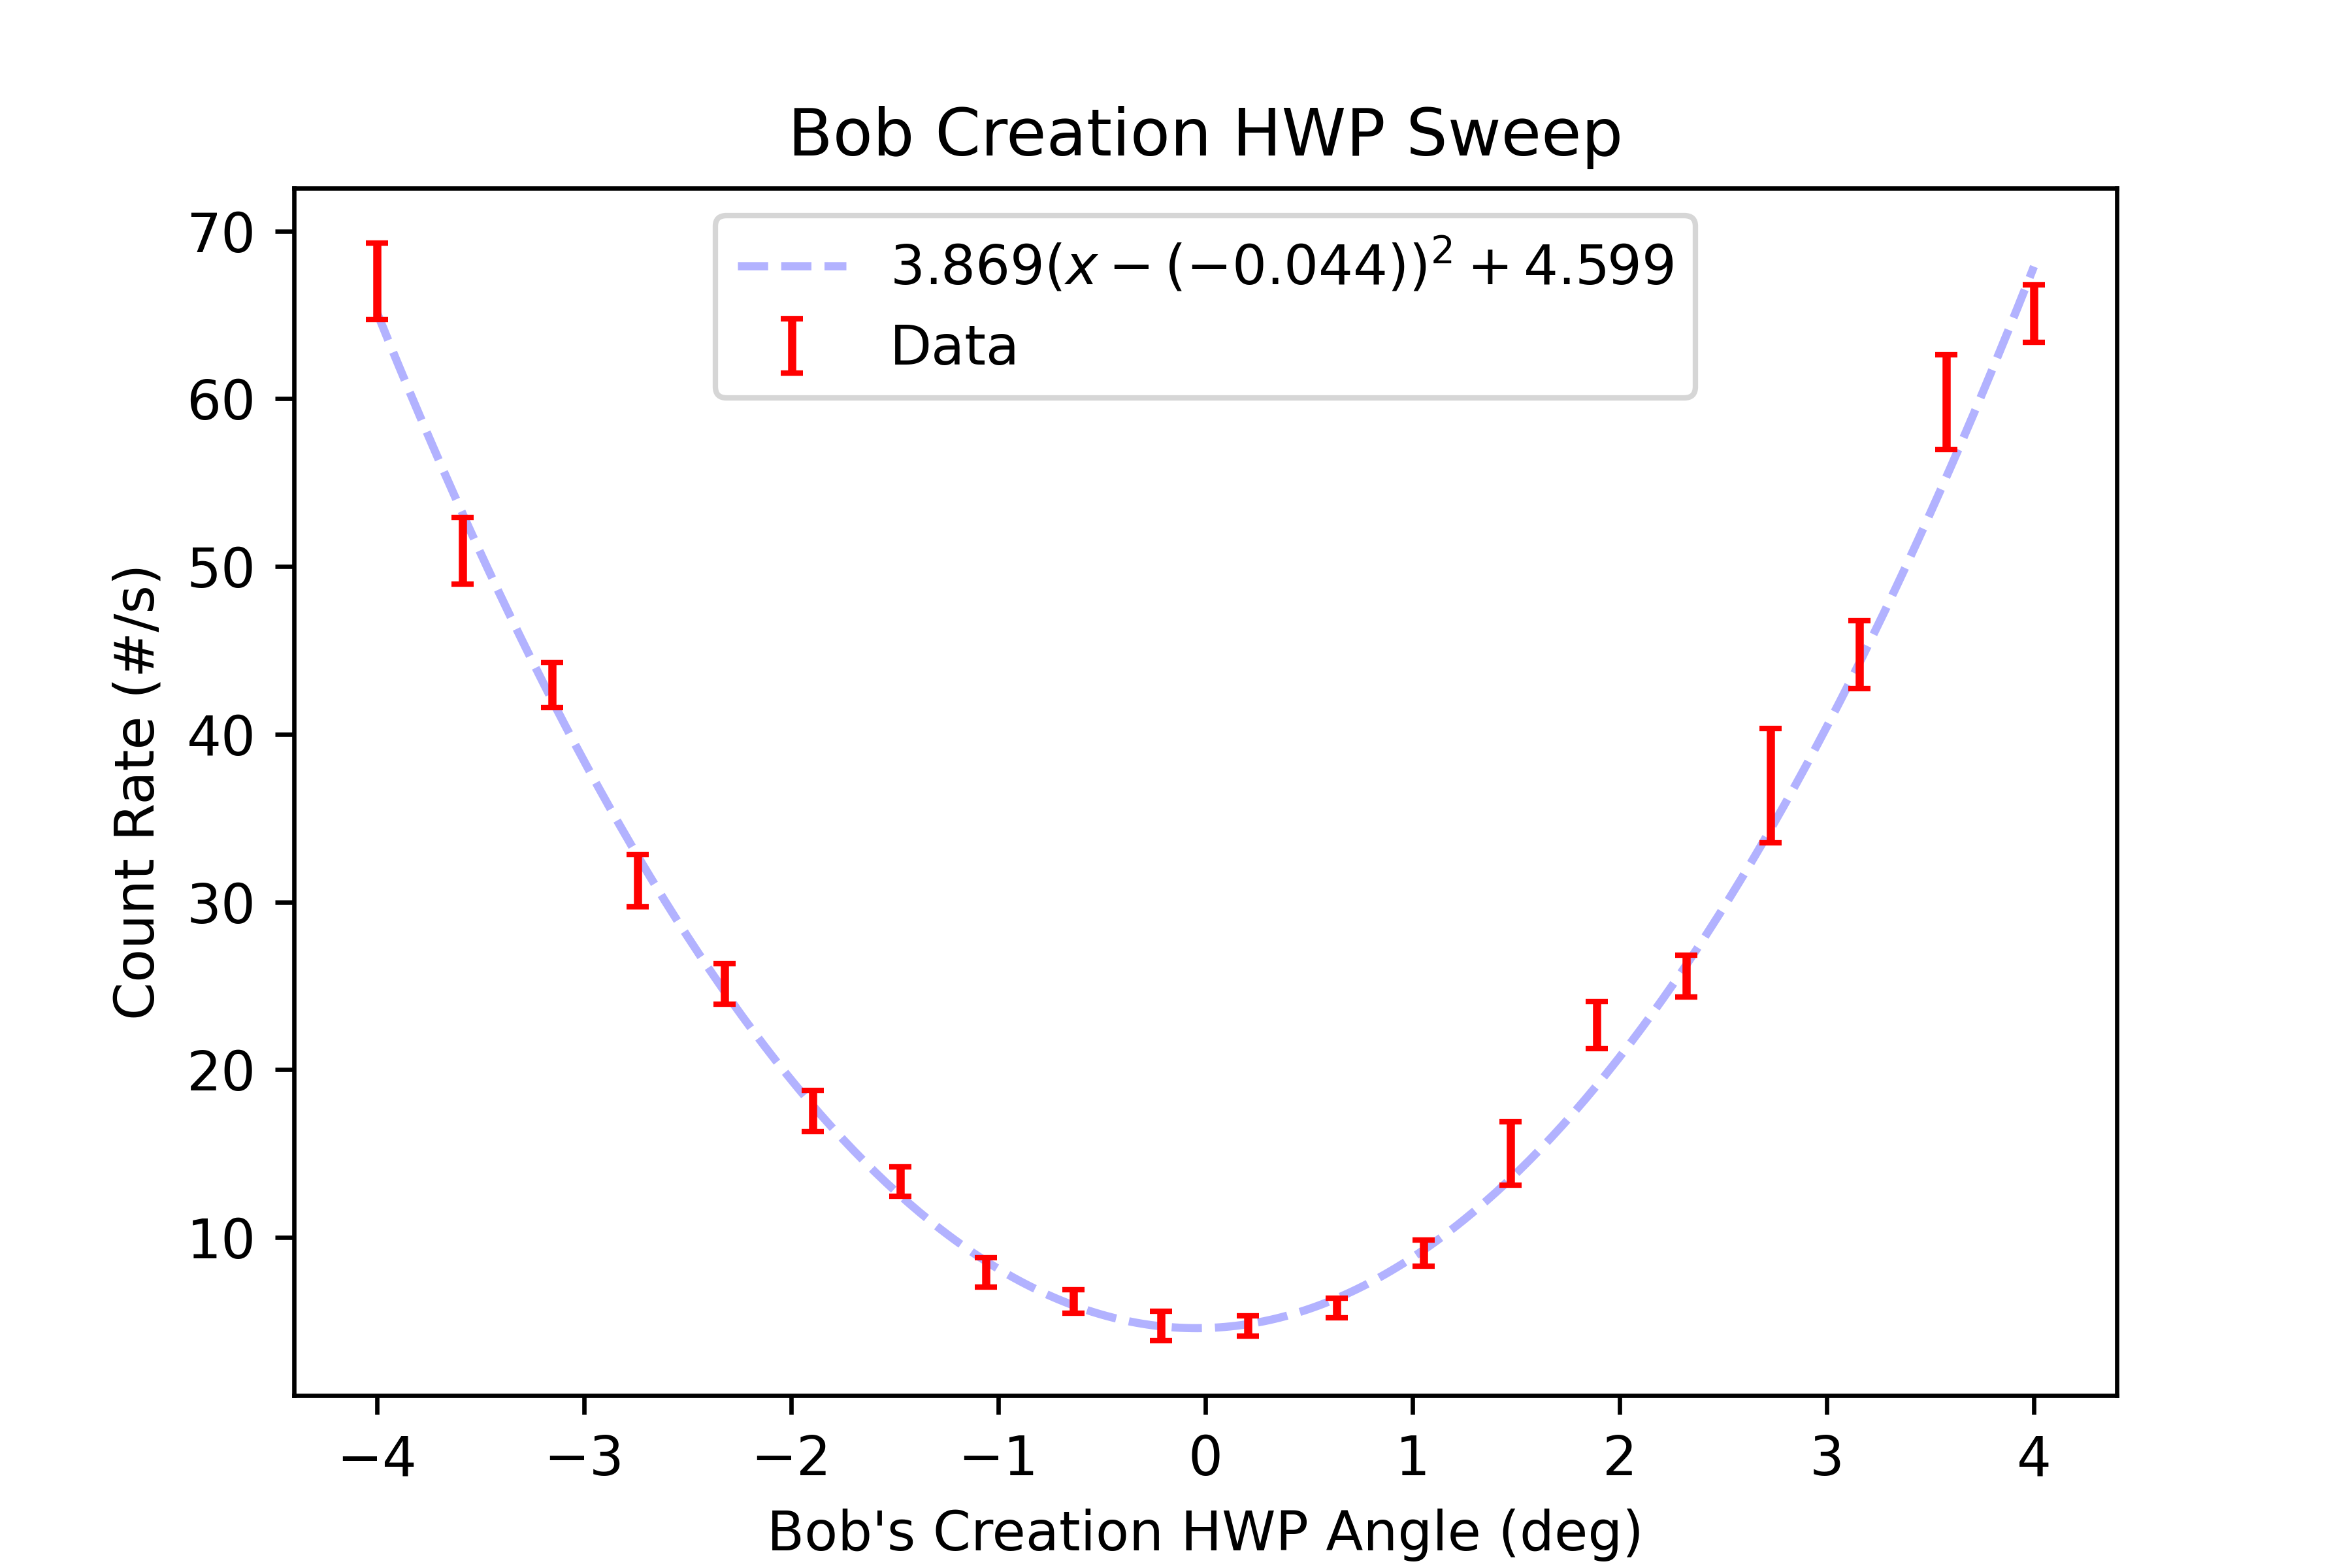
\includegraphics[width=1\linewidth]{figs/BCHWP_sweep0.png}
        \caption{}
        \label{fig:BCHWP}
    \end{subfigure}
    \begin{subfigure}{0.35\linewidth}
        \centering
        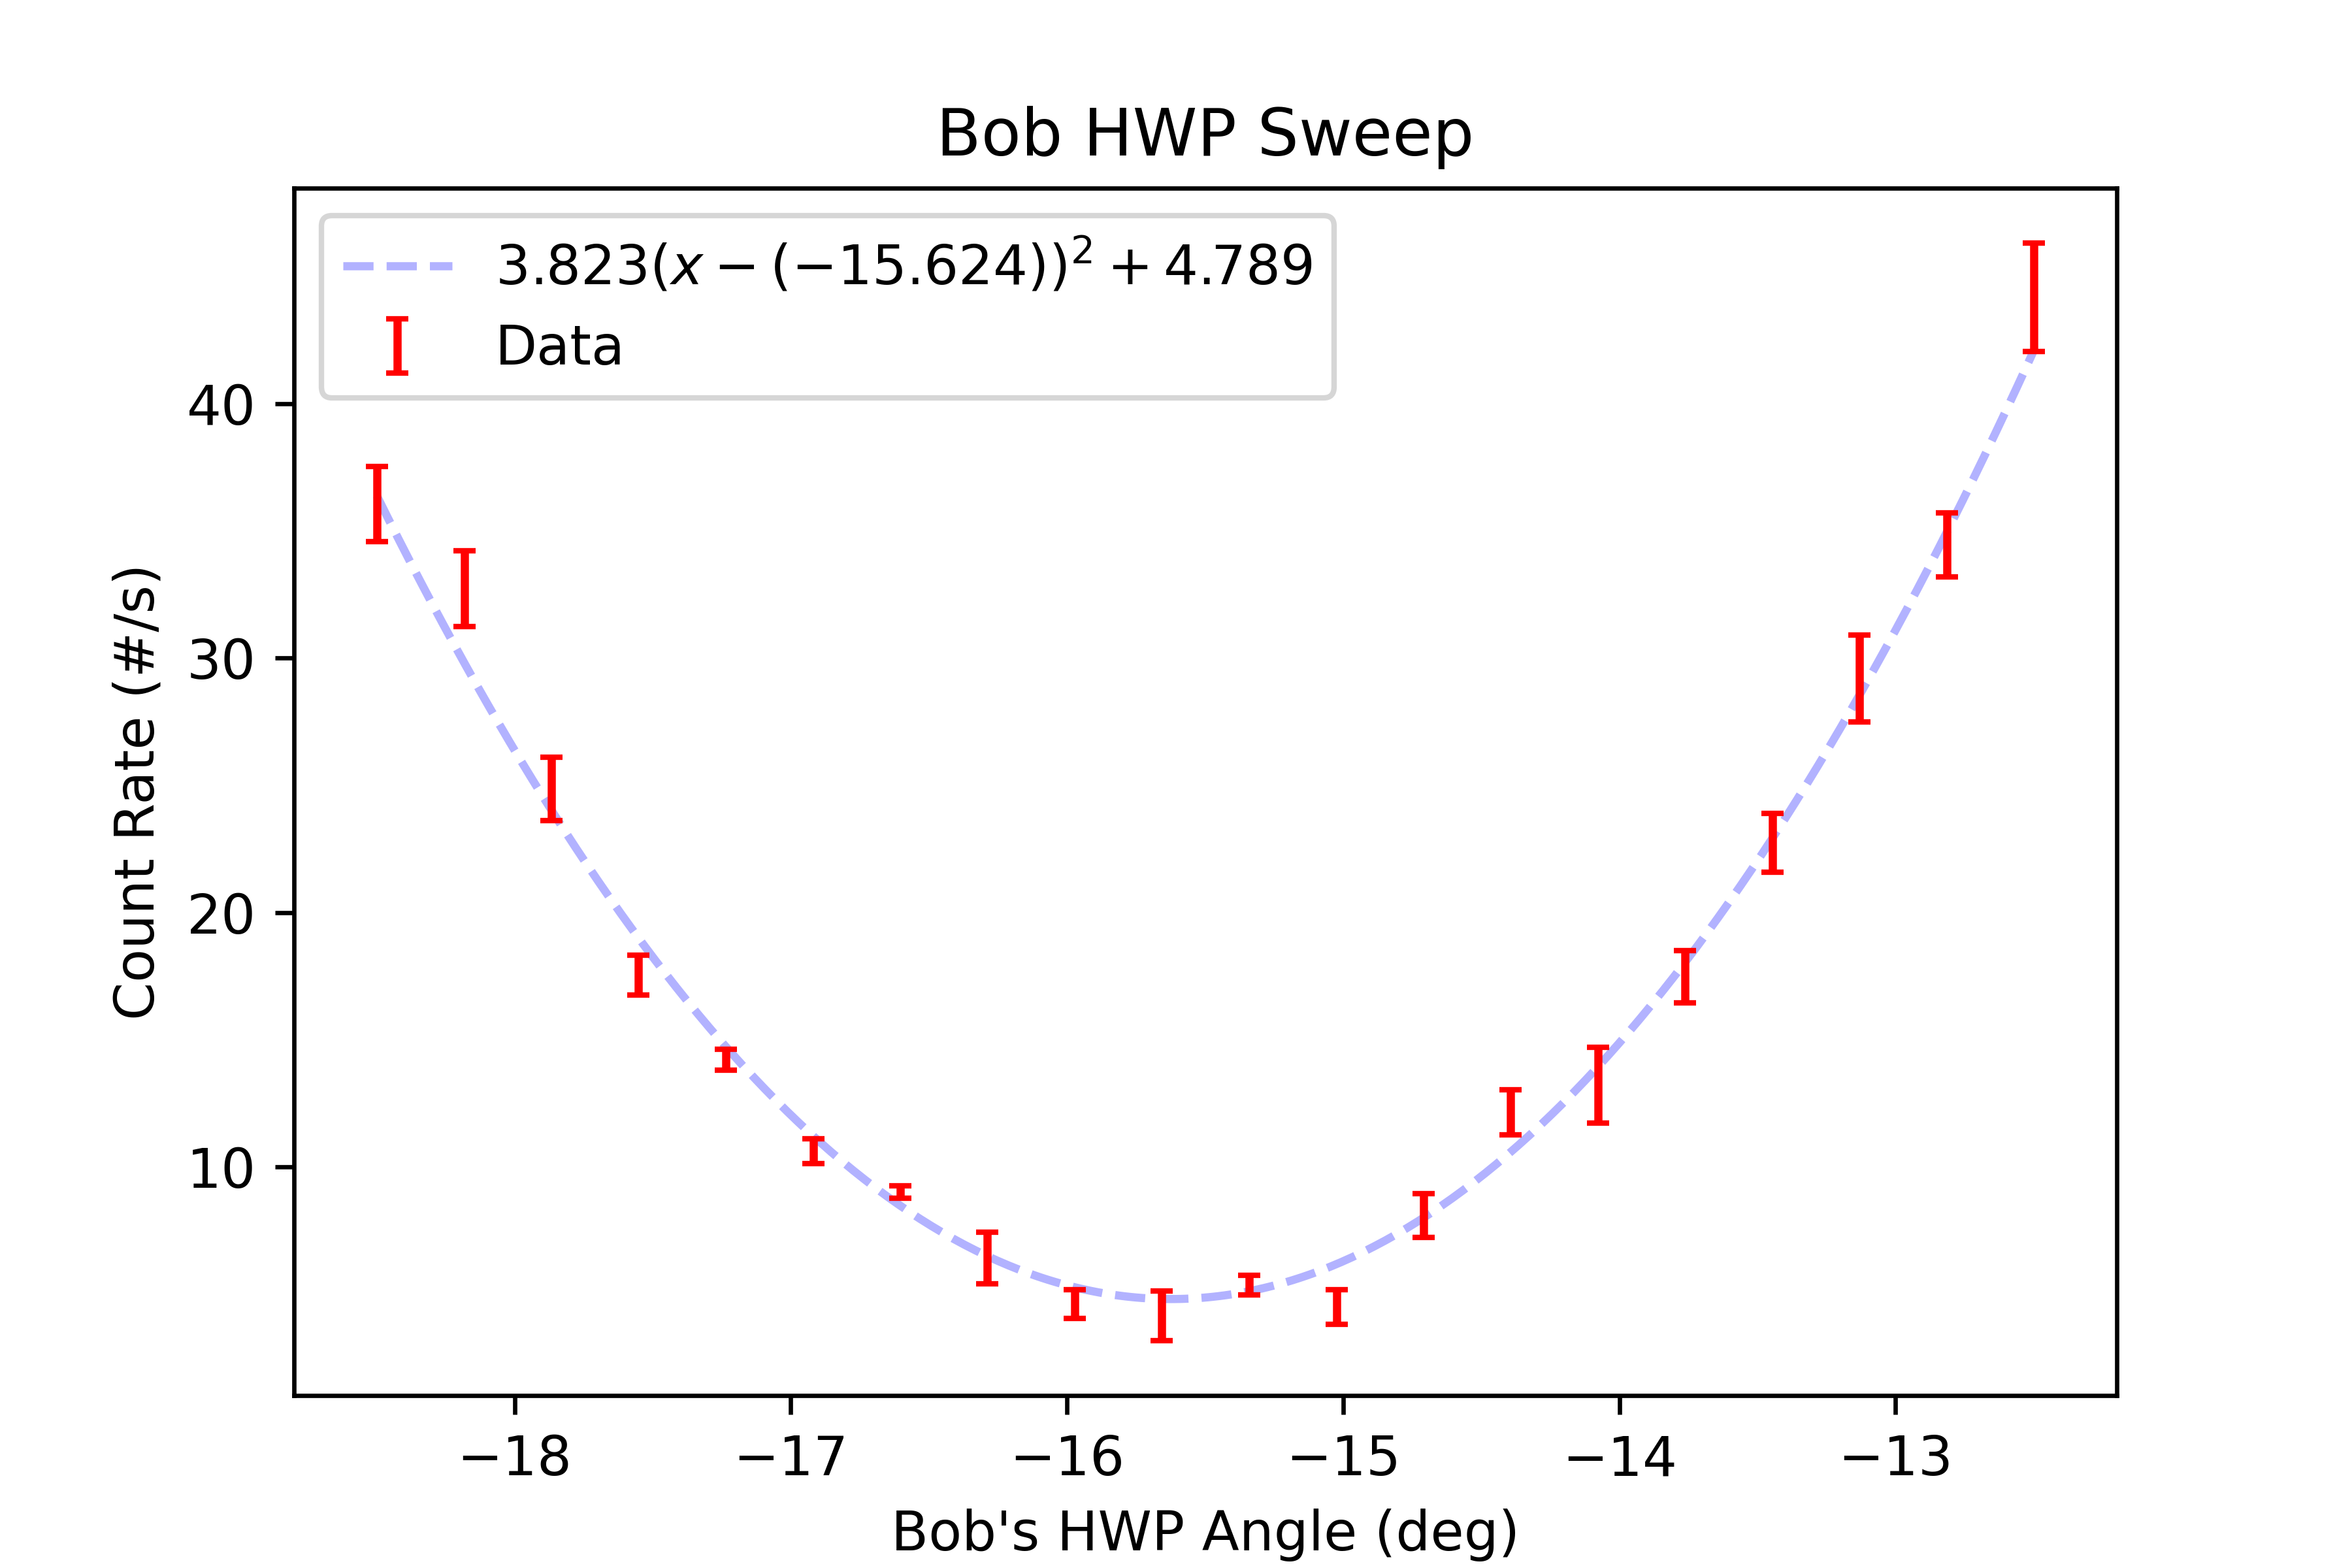
\includegraphics[width=1\linewidth]{figs/BHWP_sweep2.png}
        \caption{}
        \label{fig:BHWP}
    \end{subfigure}
    \begin{subfigure}{0.27\linewidth}
        \centering
        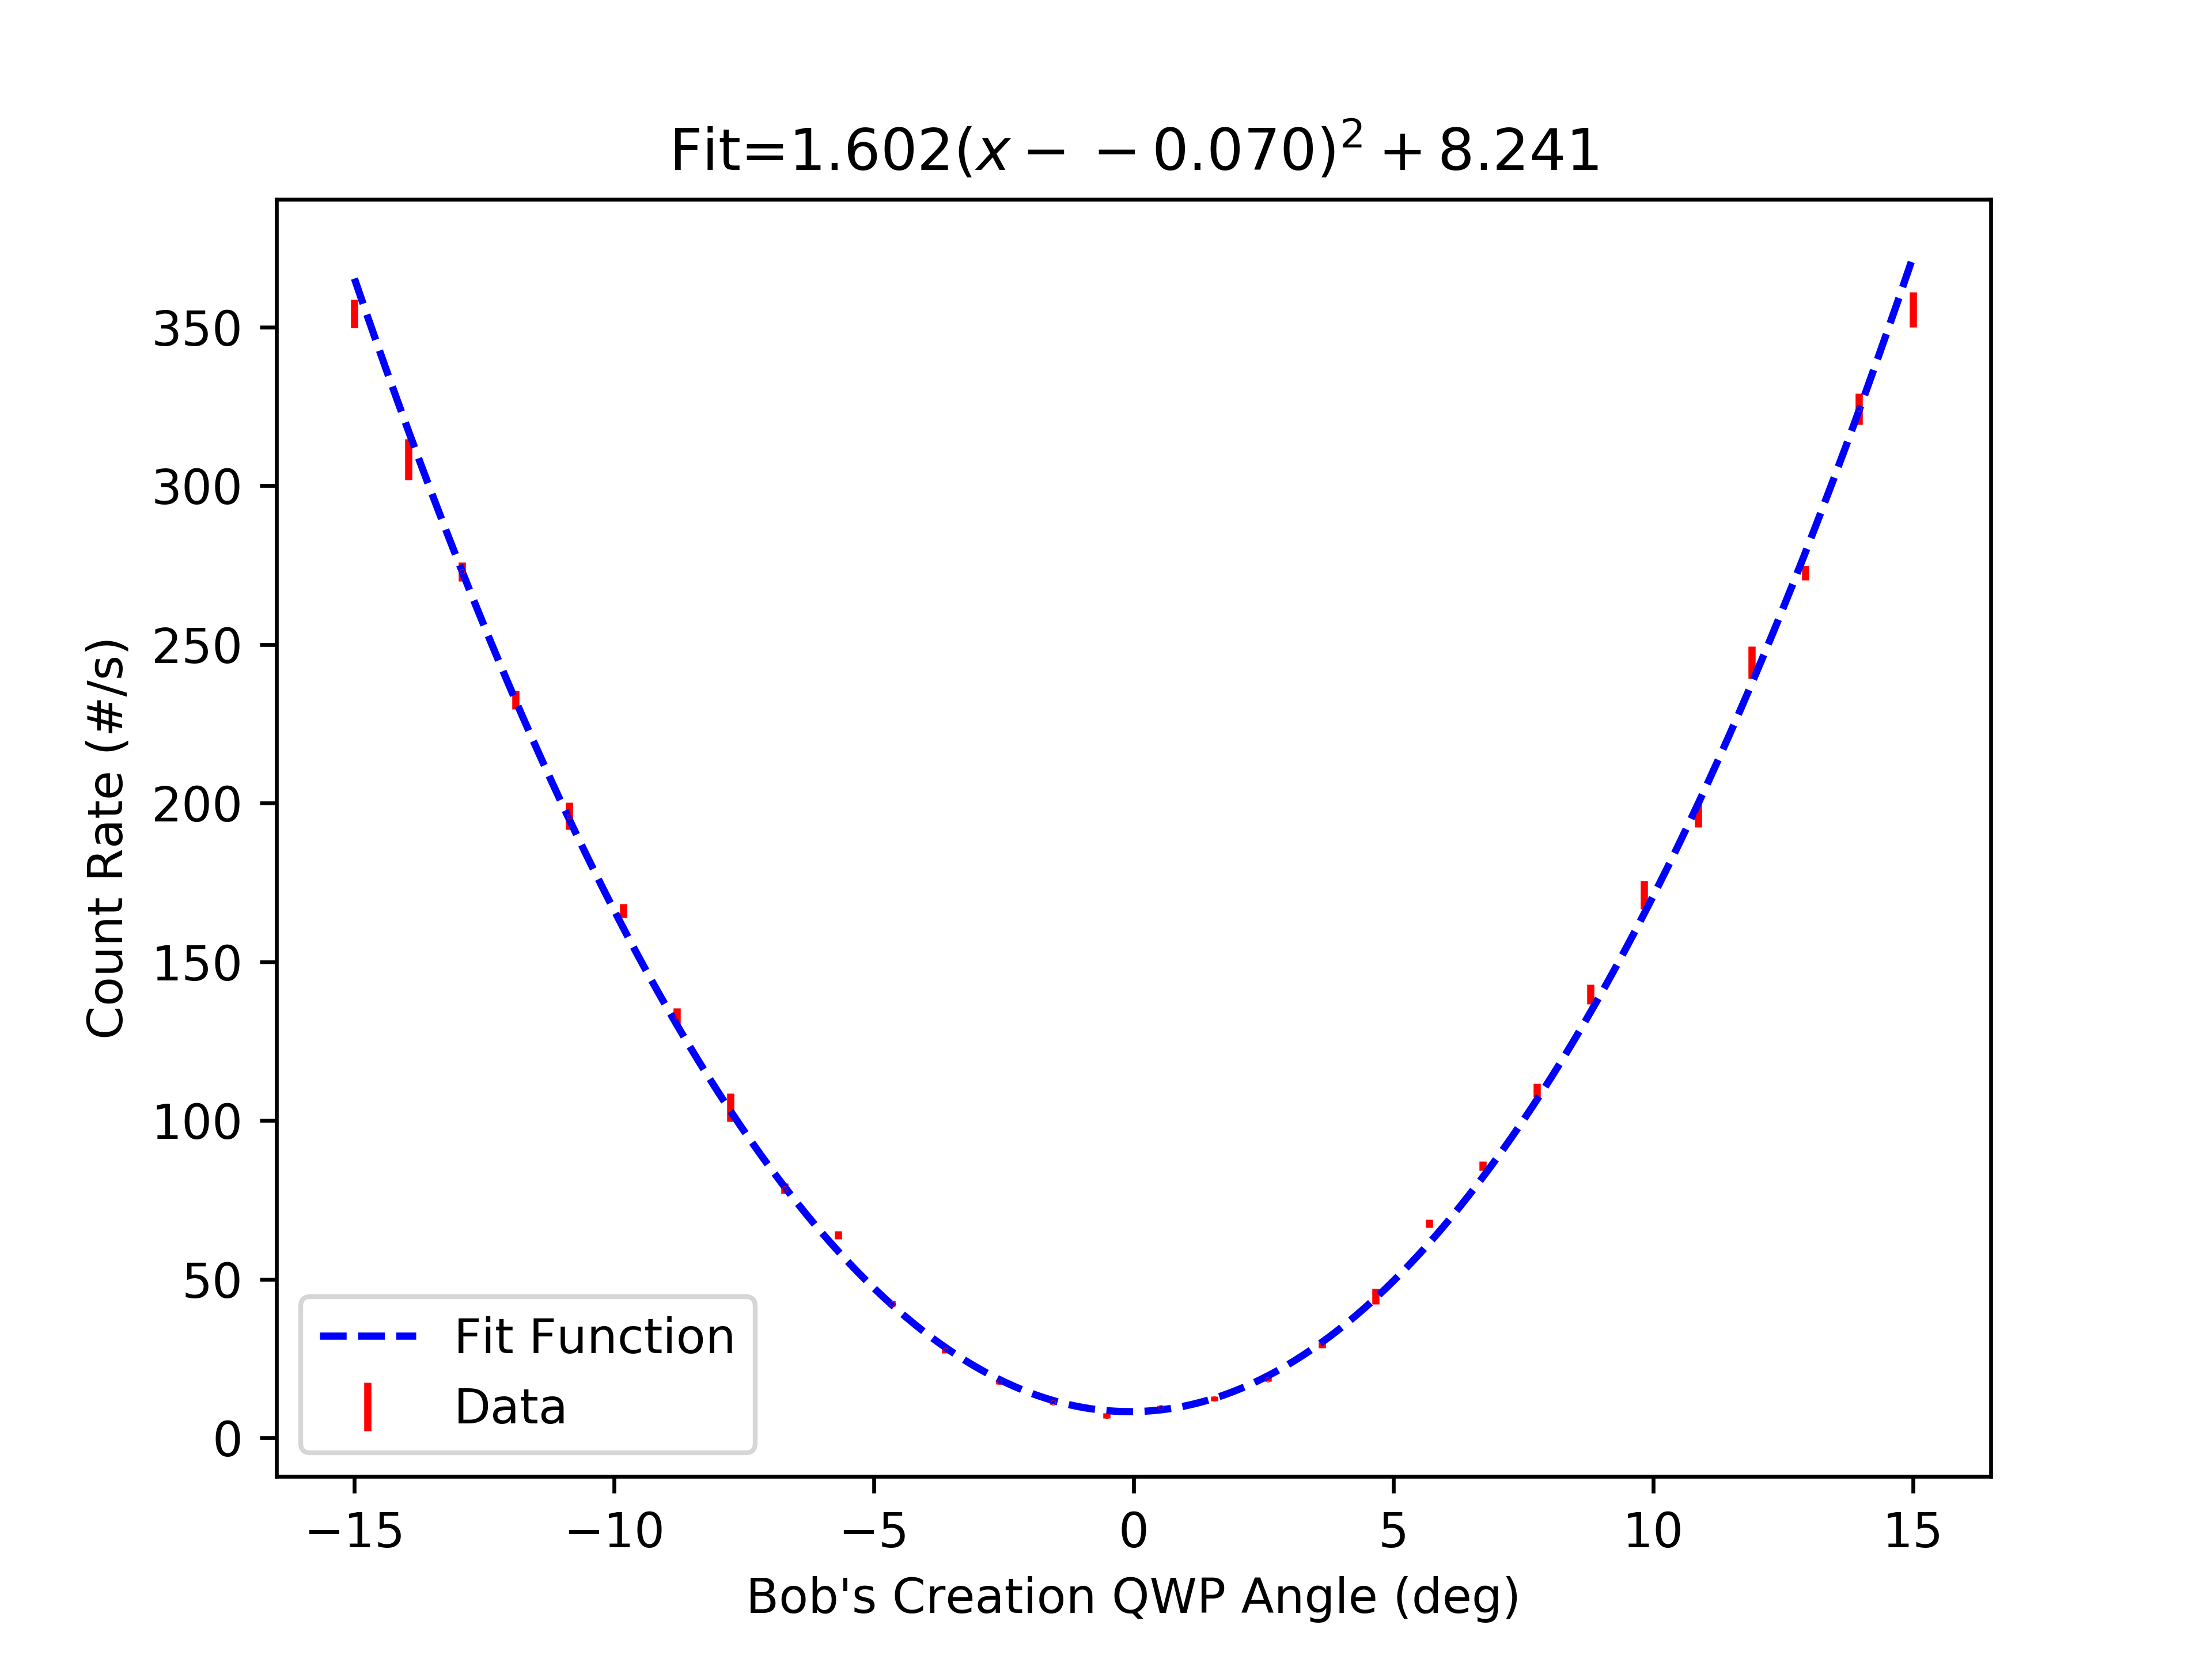
\includegraphics[width=1\linewidth]{figs/BCQWP2.png}
        \caption{}
        \label{fig:BCQWP}
    \end{subfigure}
    \caption{Top left to bottom right: BQWP calibration curve, BCHWP calibration curve, BHWP calibration curve, BCQWP calibration curve.}
\end{figure}

\begin{figure}[!]
    \centering
    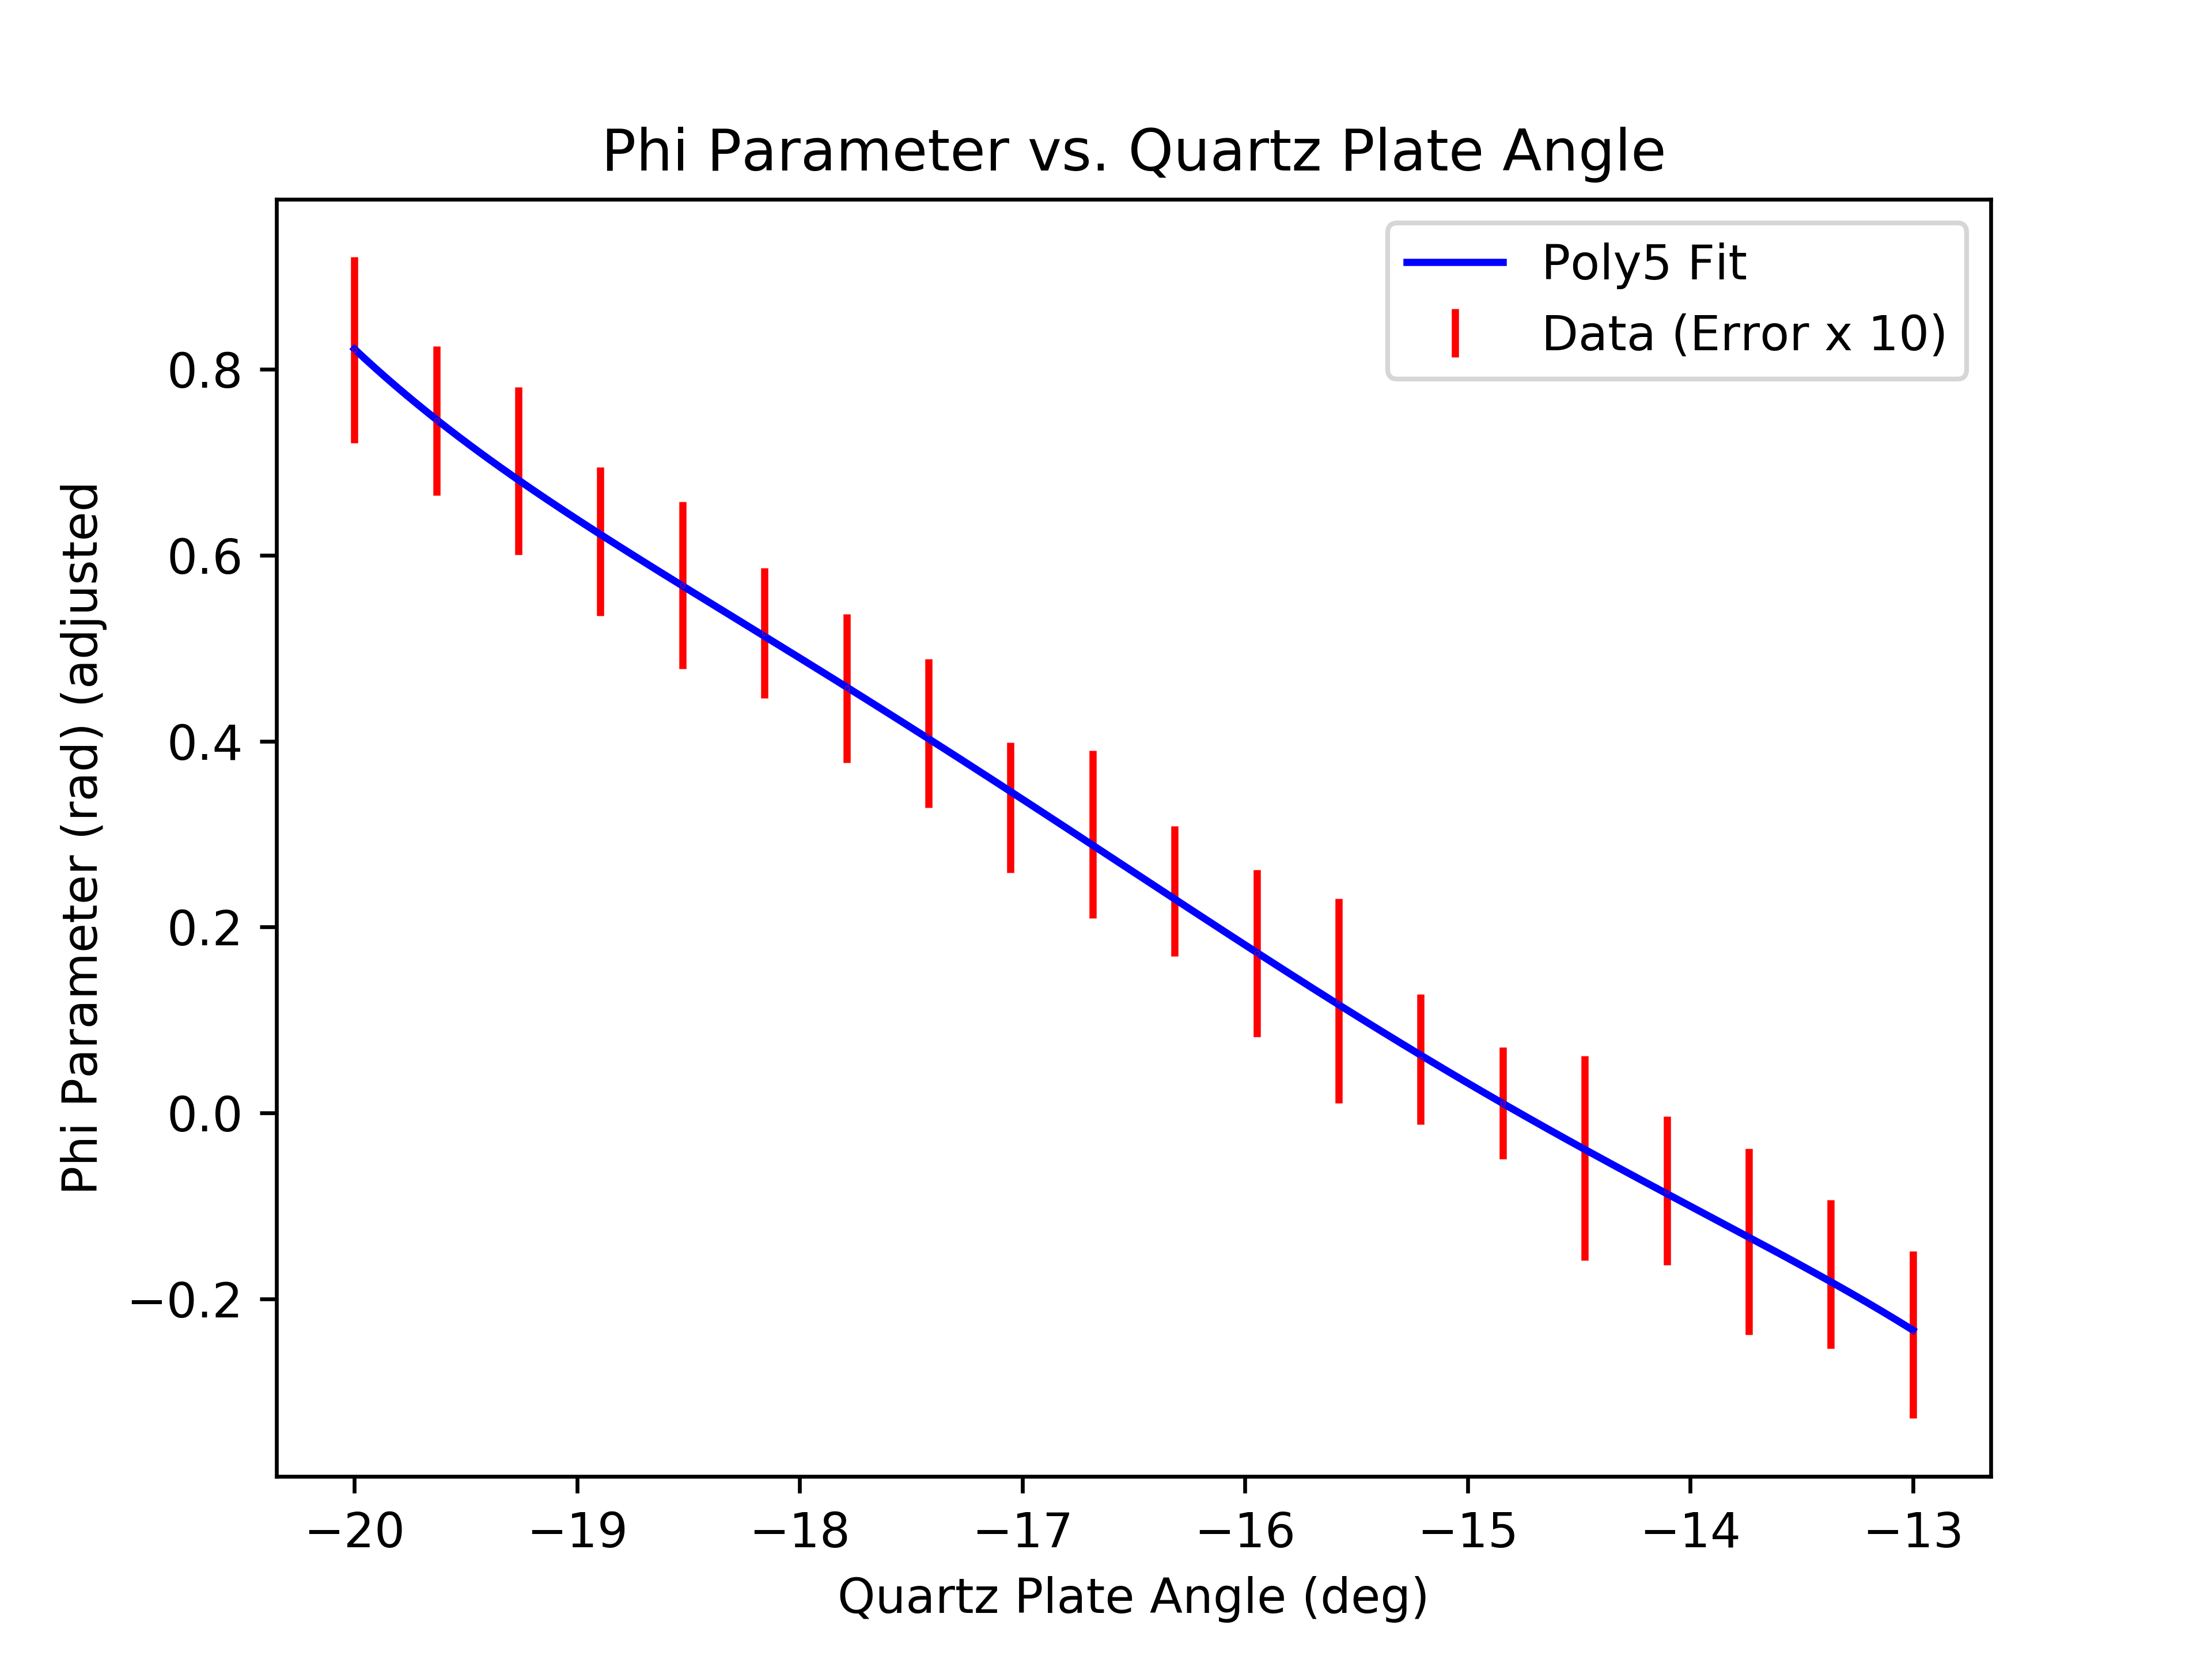
\includegraphics[width=0.75\linewidth]{figs/phi_sweep_7022024_2.png}
    \caption{Result of phase\_finding.py once run through qp\_plotting.py}
    \label{fig:phase_finding}
\end{figure}
Finally, we will calibrate the bell state $$\ket{\Phi^+} = \frac{1}{\sqrt{2}}\ket{HH} + \frac{1}{\sqrt{2}}\ket{VV},$$ as it is useful for various experiments. We will also calibrate the precompensation crystal (PCC).
\subsection{Phi Plus and the PCC}
Calibration of phi plus and the PCC is a three step process:
\begin{enumerate}
    \item Run ratio\_tuning.py, which balances the HH and VV counts to yield the even superposition wanted by phi plus. Input the value it provides into the config under the phi\_plus section. Note the plot for this specific file is not used.
    \item Run phase\_finding.py, which finds where the phase between terms is zero. Then, you can run qp\_plotting.py to generate a fitted plot of this data; you can zoom into the zero on the plot and insert that degree value into the config for phi\_plus. Note, you may sometimes receive a plot that seems to have a discontinuity in it. If this occurs, add $\pi$ to all negative phi terms in the csv and subtract $\pi$ from all positive phi terms in the csv. The plot should now look as in Figure \ref{fig:phase_finding}.
    \item Run ratio\_tuning.py again, as adjusting the QP will likely have an effect on the superposition. 
    \item Run pcc\_sweep.py, which calculates the purity of the state. Purity is a measure of how well we've created the state phi plus and is defined by $$p = \frac{<DD> + <AA> - <AD> - <DA>}{<DD> + <AA> + <AD> + <DA>}.$$ PCC sweep will calculate the purity at various PCC angles--you can then look at the csv where these values are saved and choose the PCC degree value corresponding to the highest purity--this can be put in config.json under phi\_plus as well. We aim for a purity $>0.95$. Note that purity is dependent on lab temperature (aim for $<20^\circ C$) and how long the laser has been on for (wait at least 10 minutes from when the laser is turned on). This is an iterative process.
\end{enumerate}

You are now ready to run experiments! Note that these files can be used to calibrate $\ket{\Phi^-}$ as well, given an adjustment to the UVHWP sweep in ratio\_tuning of 45 degees. 

\section{Random Issues with the Apparatus}
The number one thing to remember whenever an error occurs is to first run 'm.shutdown()' in the terminal if the Manager has been instantiated. This resets all wave plates to their calibrated zeros and removes the risk of losing calibrations. See how to instantiate the manager from terminal in section \ref{sec:calib_not_from_scratch}.

\subsection{The Quartz Plate Refusing to Move}
Sometimes, the QP will return the error 'RuntimeError: Sent instruction "b'Bma0001FB24'" to ElliptecMotor-C\_QP expecting response length 11 but got response b'BGS0A' (length=5). As of writing, we have mostly resolved this issue by allowing the QP to be attached to its own bus (COM12), such that whenever it loses connection/bugs out we can reset it in this order: remove USB from usb hub, remove power supply cable from bus, remove ribbon cable, replace ribbon cable, replace power supply cable, replace USB. We then recalibrate as per section 2.
\subsection{COM5/7 Refusing to Open}
Make sure you've run m.shutdown() if the Manager was initialized. Then, run the Task Manager program on the PC and kill VS Code. Open VS Code again and try your program. If it still does not work, you can enter Ello, connect to the COM in question, disconnect, close Ello, and try running your file again. Sometimes, a simple quit() followed by ipython works, but not always.
\subsection{Serial Number Errors}
Sometimes the Thorlabs motors connected to the measurement wave plates will lose connection with the computer--this is recognized by an error in the Python terminal similar to "Internal serial number is incorrect", and identified by closing VS Code, opening APT User, and seeing some or all of the motors missing from the home page. Assuming that the motors had been homed before this error and are at their visual zero, this can be fixed by: Closing APT User, unplugging the motor block at their base, opening APT User with motors unplugged, closing it again, plugging back in the motor bases and waiting until all four have a green LED, opening APT User, and verifying there that all four motors now show there. 

If the motor is not set to zero and not visible in APT User, you can try manually jogging it on its base to see if it is recognized. If not, I am sorry you have to unplug, replug as described above then recalibrate as in section 2.
\subsection{Fitting Errors}
As each fiting error is different, we describe here general troubleshooting steps:
\begin{enumerate}
    \item During a QP sweep $\rightarrow$ often the bounds are set too wide, such that the QP itself blocks the light at certain points. Print out the sweep right before fitting and you should see this occuring at the boundary. Fix by narrowing bounds.
    \item Sometimes we will be sweeping the QP while in the wrong UV HWP quadrant--this will result in a maxima where a minima would otherwise be. Resolve this by adding 45 degrees to the UV HWP value you are using (either $\ket{\Phi^+}$ or $\ket{\Phi^-}$ pending what state you are starting from) in the program, then setting it back to the wanted value post-sweep.
    \item Anything else? Best advice I can give is to \textit{print()} the sweep results. Good luck!
\end{enumerate}
\section{Calibration not from Scratch}\label{sec:calib_not_from_scratch}
Here I will describe various \textit{extremely} useful terminal/Python commands for the Manager object that will be helpful for troubleshooting and calibrating the setup. They are:
\begin{enumerate}
    \item 'from lab\_framework import Manager' $\rightarrow$ imports the Manager framework into your file or terminal.
    \item 'm = Manager(config = './config.json')' $\rightarrow$ sets the Manager object as m. The CCU will automatically start displaying data. You may need to adjust the number of dots pending what directory you're in.  
    \item 'm.OBJECT\_goto(value) $\rightarrow$, where OBJECT is named as in your config.json and value is 0 to 360. An example is 'm.C\_UV\_HWP.goto(22.5)'.
    \item 'm.take\_data(num-points, time-per-point)' $\rightarrow$ takes data into the Manager object, example is 'm.take\_data(5,3).
    \item 'm.shutdown()', shuts down the Manager object and returns all wave plates to their calibrated zero. This must be run anytime you are done taking data or moving wave plates. 
\end{enumerate}
These can be used to mimic much of the functionality of individual calibration files, allowing you to calibrate individual components that may have broken without repeating the entire process! 

\subsection{Github (Please Push)}
We use a Git Bash terminal to push all files and experimental data to and from the cloud. It is best practice to 
\begin{enumerate}
    \item cd Summer\_2024/ (or whatever repo your work is in)
    \item git pull
\end{enumerate}
when starting your day's work. At end of day,
\begin{enumerate}
    \item cd Summer\_2024/ (or whatever repo your work is in)
    \item git add .
    \item git commit -m "descriptive note of what you're pushing"
    \item git push
\end{enumerate}
to ensure all data and files are available online for future work. Github is super useful for keeping track of your results, code, and writing, and ensures good experimental practice. 
\end{document}